\documentclass{beamer}

\usepackage[fontset=none]{ctex}
\usepackage{listings}
\usepackage{geometry}
\usepackage[shortlabels]{enumitem}
\usepackage{fancyvrb}
\usepackage{graphicx}

\lstset{language=TeX,
    numbers=left,
    numberstyle=\tiny,
    keywordstyle=\color{blue!70},
    commentstyle=\color{red!50!green!50!blue!50},
    frame=shadowbox,
    rulesepcolor=\color{red!20!green!20!blue!20}
}

\setCJKmainfont[BoldFont={FZCSJ.otf},
    ItalicFont={FZKTJ.otf},
    BoldItalicFont={FZCKJ.otf}]{FZSSJ.otf}
\setCJKsansfont[AutoFakeSlant,AutoFakeBold]{FZHTJ.otf}
\setCJKmonofont{FZFSJ.otf}

\AtBeginSection[]{
    \begin{frame}
        \tableofcontents[currentsection,hideallsubsections]
    \end{frame}
}

\usetheme{Berlin}
\usefonttheme[onlymath]{serif}

\title{高速\LaTeX{}入门课程}
\author{曾梦辰}
\institute{北京师范大学OM学社}
\date{最后编译:\ \today}

\begin{document}
\maketitle

\begin{frame}
    \frametitle{目录}
    \tableofcontents
\end{frame}

\section{前言}

\begin{frame}
    \frametitle{关于\LaTeX{}}
    LaTeX (读作Lah--tek或Lay--tek, 不要读成Lay--teks), 是一种基于TeX的排版系统, 由美国计算机科学家Leslie Lamport在20世纪80年代初期开发.
    利用这种格式系统的处理, 即使用户没有排版和程序设计的知识也可以充分发挥由TeX所提供的强大功能, 不必一一亲自去设计或校对, 能在几天, 甚至几小时内生成很多具有书籍质量的印刷品生成复杂表格和数学公式, 这一点表现得尤为突出.
    因此它非常适用于生成高印刷质量的科技和数学, 物理文档.
    这个系统同样适用于生成从简单的信件到完整书籍的所有其他种类的文档.

    LaTeX使用TeX作为它的格式化引擎, 当前的版本是\LaTeXe.\pause
    \vspace{1cm}
    以上是抄的维基百科.
\end{frame}

\begin{frame}
    \frametitle{参考资料}
    我们推荐一些可以阅读的参考资料.\pause
    \begin{itemize}
        \item<2-> Overleaf.\ \emph{Learn LaTeX in 30 minutes}.
        (本幻灯片的主要参考资料, 不过没有汉语翻译.)
        \item<3-> Tobias Oetiker, et.~al.\ \emph{一份 (不太) 简短的\LaTeXe{}介绍}.
        (可能是最好的入门教材.)
        \item<4-> Frank Mittelbach, Ulrike Fischer.\ \emph{The \LaTeX Companion}, 3rd Edition.
        (将近两千页的大肥书, 可以挑着看, 不要试图看完.)
        \item<5-> 本幻灯片. 用法: 使用Acrobat或者你喜欢的PDF阅读器, 然后利用鼠标左键/鼠标滚轮/幻灯片右下角的按钮进行翻页.
    \end{itemize}
\end{frame}

\begin{frame}
    \frametitle{听完本次课程后, 你将会\dots}
    \begin{enumerate}[(1)]
        \setcounter{enumi}{-1}
        \item \emph{能够}科学使用搜索引擎.
        \item 学会如何使用Overleaf或者\TeX{}Page进行\LaTeX{}写作.
        \item 学会编写属于自己的\emph{Hello, World!}文档.
        \item \emph{知道}怎么输入数学公式.
        \item 学会如何使用\Verb|texdoc|命令或者在\Verb|CTAN|上查找宏包文档.
        \item 从我的群里薅走一些实用书籍.
    \end{enumerate}\pause
    我觉得这些就够了.
    学习\LaTeX{}不是听一次课就能学会的, 需要自己下来勤加练习.
    有了上面这几点, 我认为已经有了一个良好的开端.
\end{frame}

\section{环境配置}

\begin{frame}
    \frametitle{\TeX{}Live的安装}
    这道题期末不考.

    感兴趣的同学可以查看文档\emph{一份简短的关于\LaTeX{}安装的介绍} (\Verb|texdoc install-latex-guide-zh-cn|, \Verb|texdoc|命令我们之后会讲到).
\end{frame}

\begin{frame}
    \frametitle{开始使用Overleaf}
    首先打开网址\url{https://cn.overleaf.com}, 看到如下页面:
    \begin{figure}[h]
        \centering
        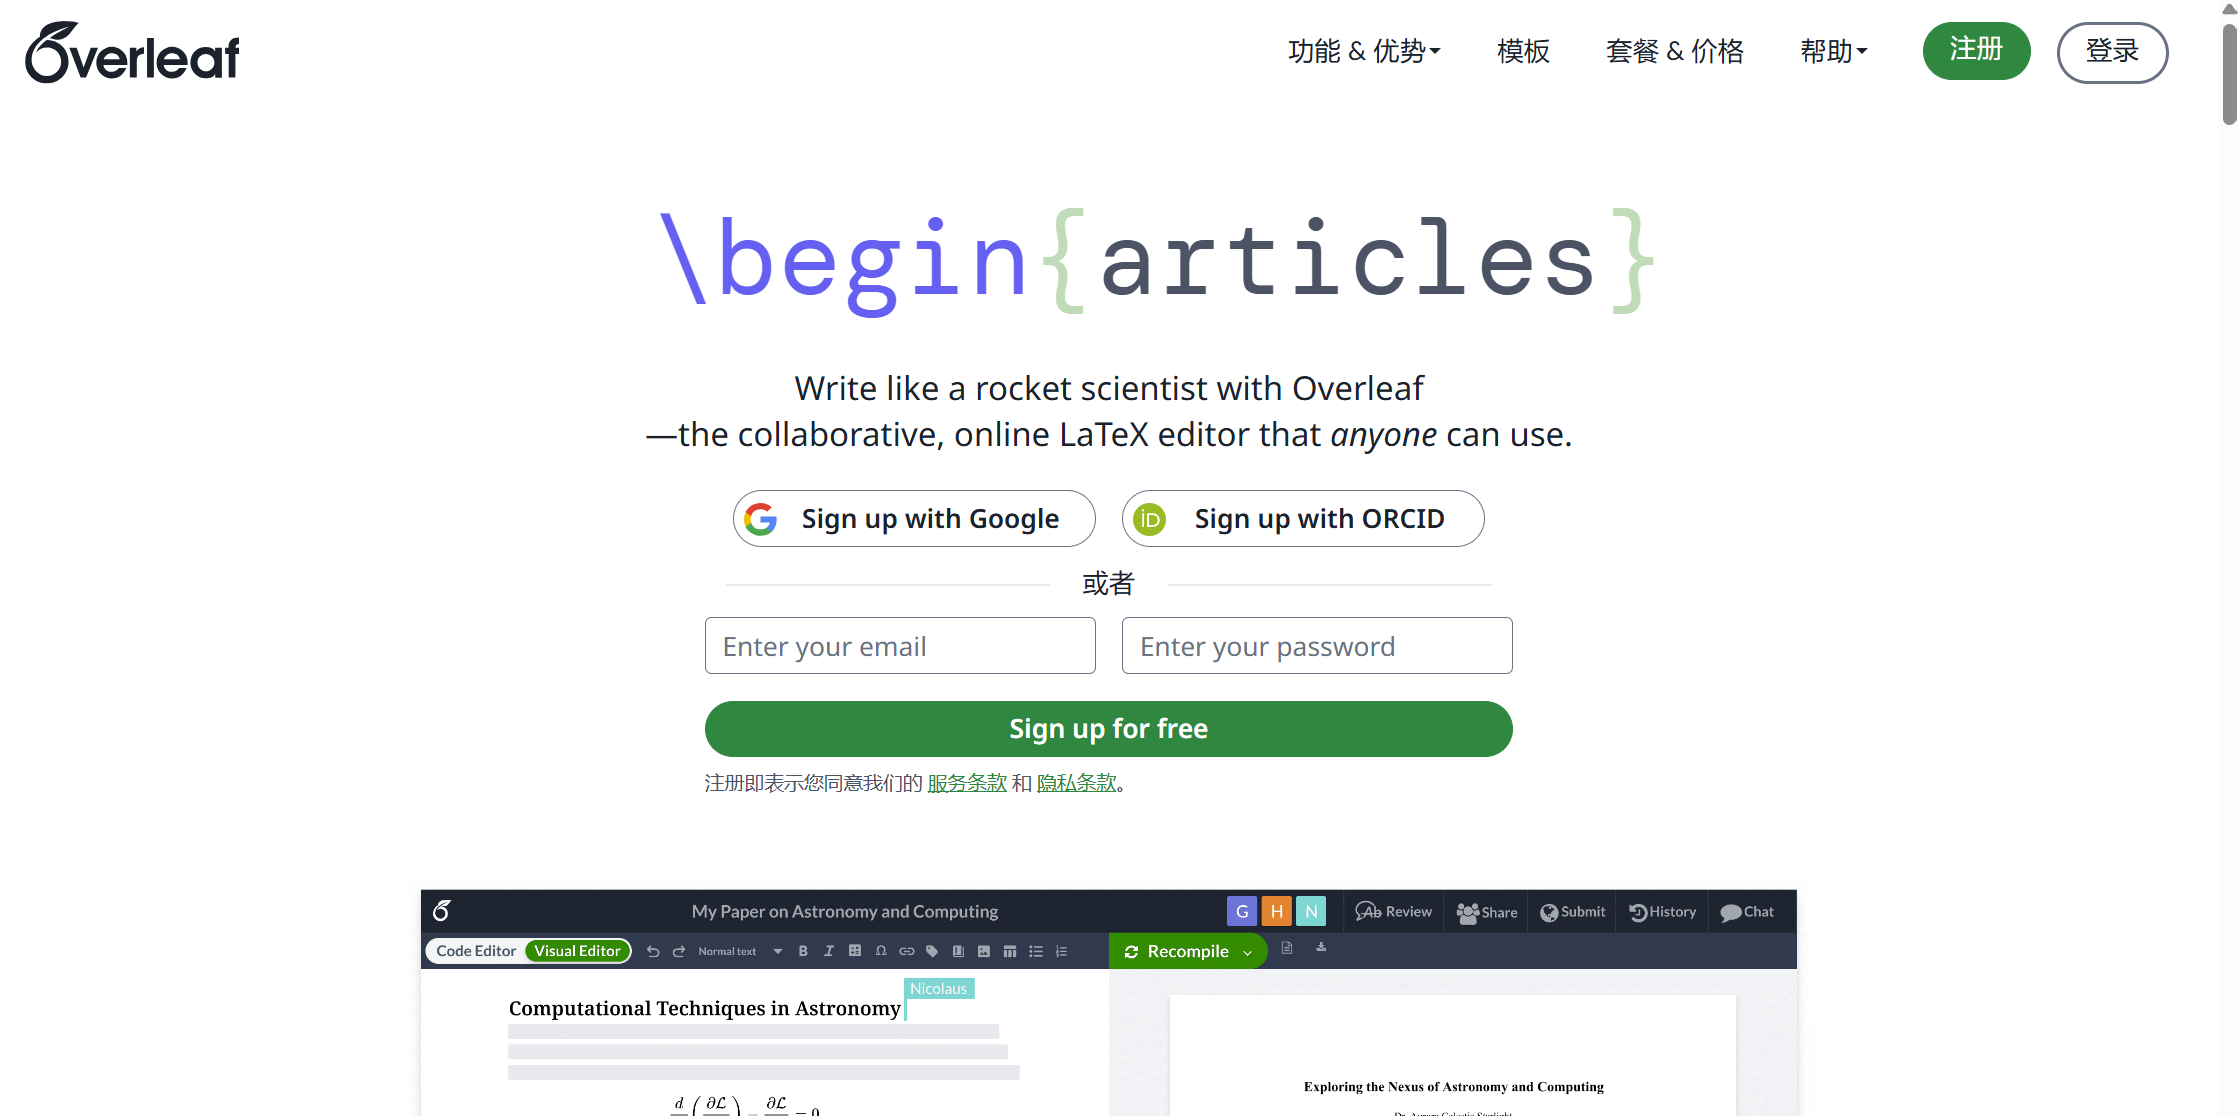
\includegraphics[width=0.8\textwidth]{figure/overleaf-signin.png}
    \end{figure}\pause
    然后在这两个方框里填写你的邮箱和你想要的密码.
    Then enjoy \LaTeX{ing}!
\end{frame}

\section{我的Hello, world!}

\begin{frame}
    \frametitle{创建第一个项目}
    现在你创建好了账号, 你应该会看到这样一个页面:
    \begin{figure}[h]
        \centering
        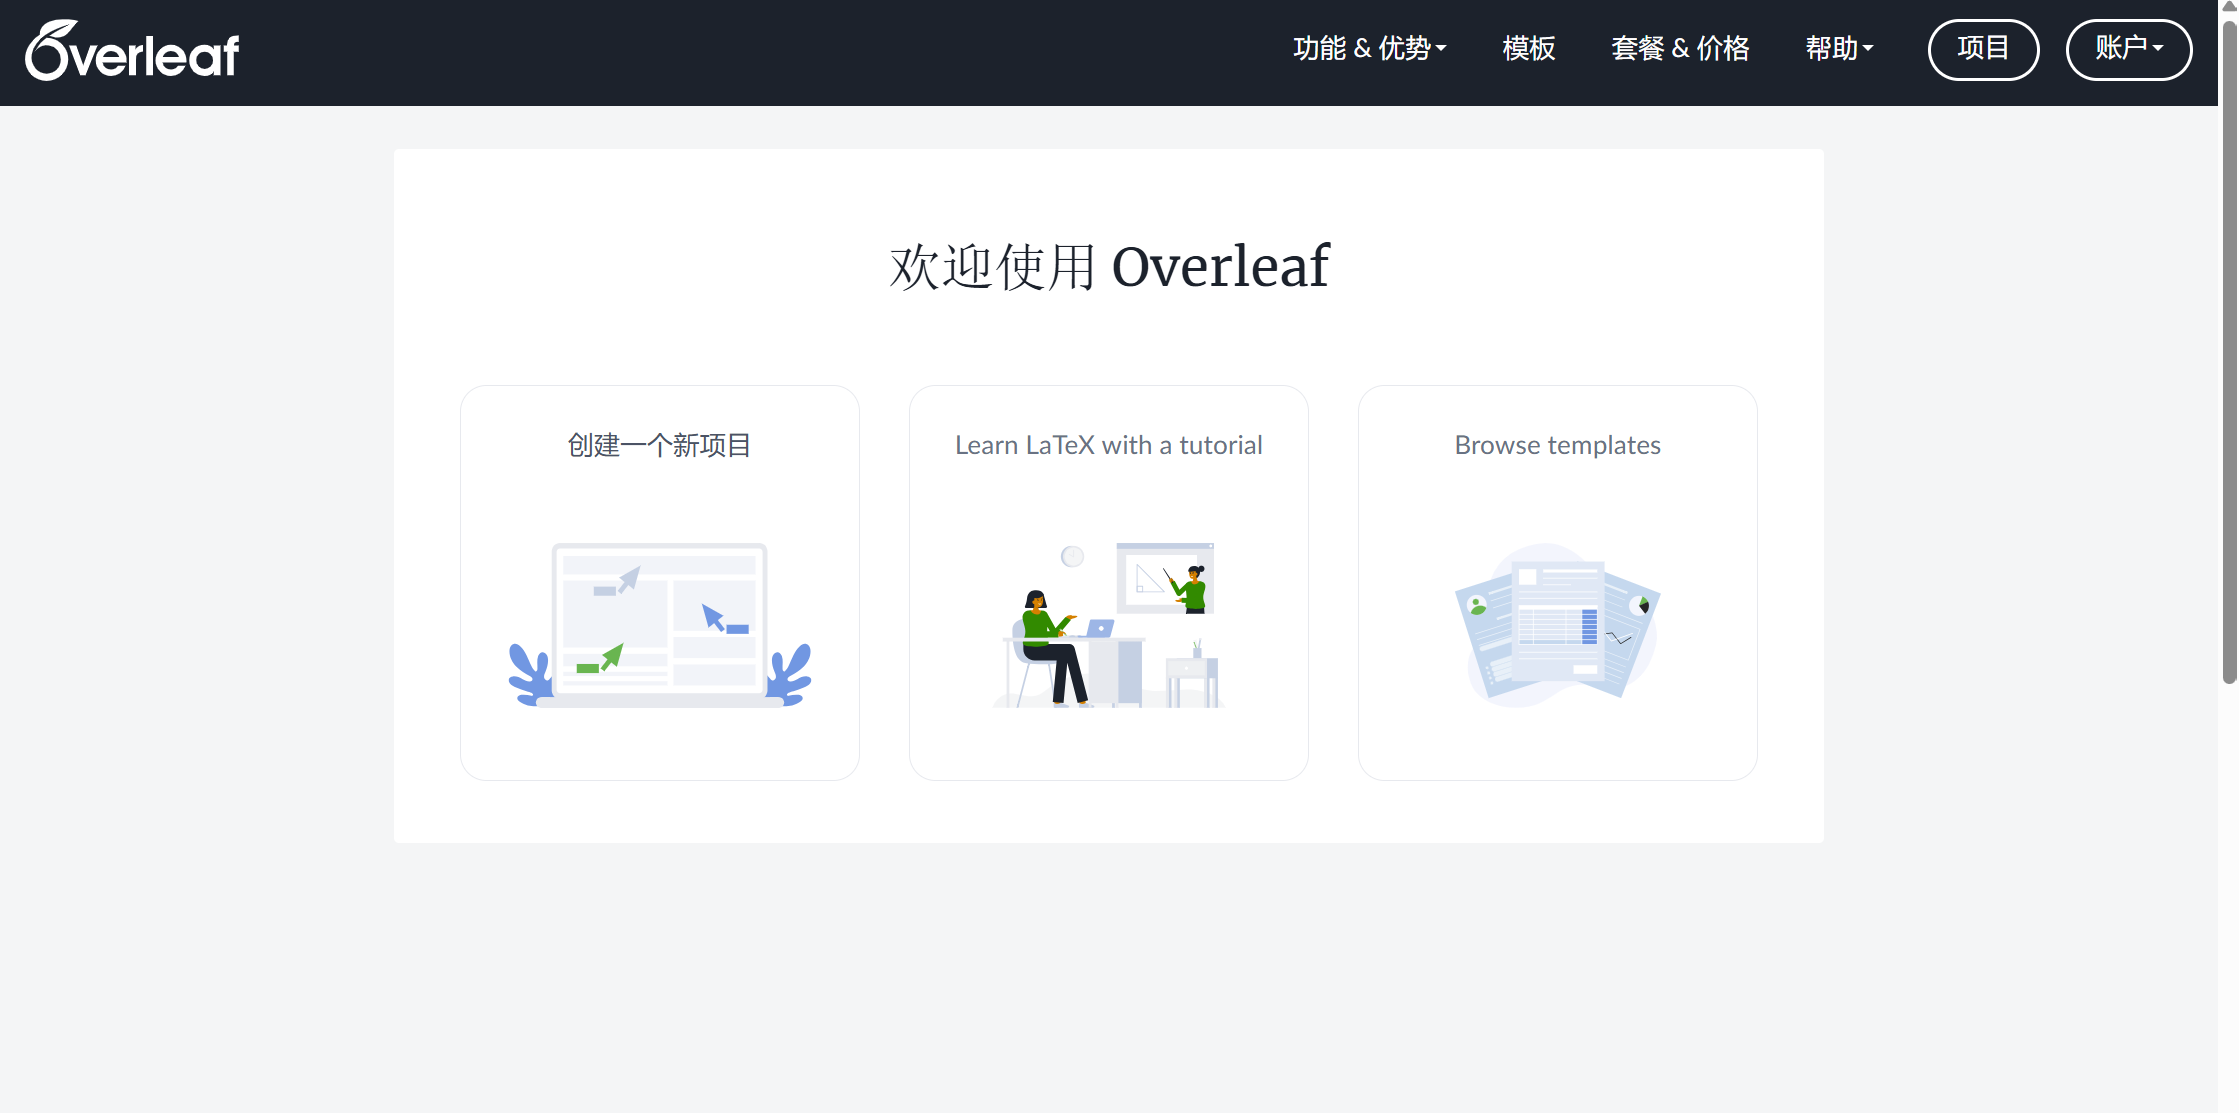
\includegraphics[width=0.8\textwidth]{figure/overleaf-startproject.png}
    \end{figure}\pause
    然后依次``创建一个新项目'', ``空白项目'', 并输入项目名称\Verb|Hello, world!|或者你喜欢的名字.\pause

    之后再创建项目的页面不长这样, 但是也很容易操作.
\end{frame}

\begin{frame}[fragile]
    \frametitle{编写Hello, world!的代码}
    把Overleaf自带的代码全部删掉, 然后输入如下的代码:
    \begin{lstlisting}
        \documentclass[12pt]{article}
        \usepackage[a4paer]{geometry}
        \title{Hello, World!}
        \author{Your name}
        \date{\today}
        \begin{document}
            \maketitle
            Hello, world! Hello, \LaTeX!
        \end{document}
    \end{lstlisting}
\end{frame}

\begin{frame}
    \frametitle{一个好习惯}
    点击左上角``菜单'', 然后如图将编译器调整为XeLaTeX.
    \begin{figure}[h]
        \centering
        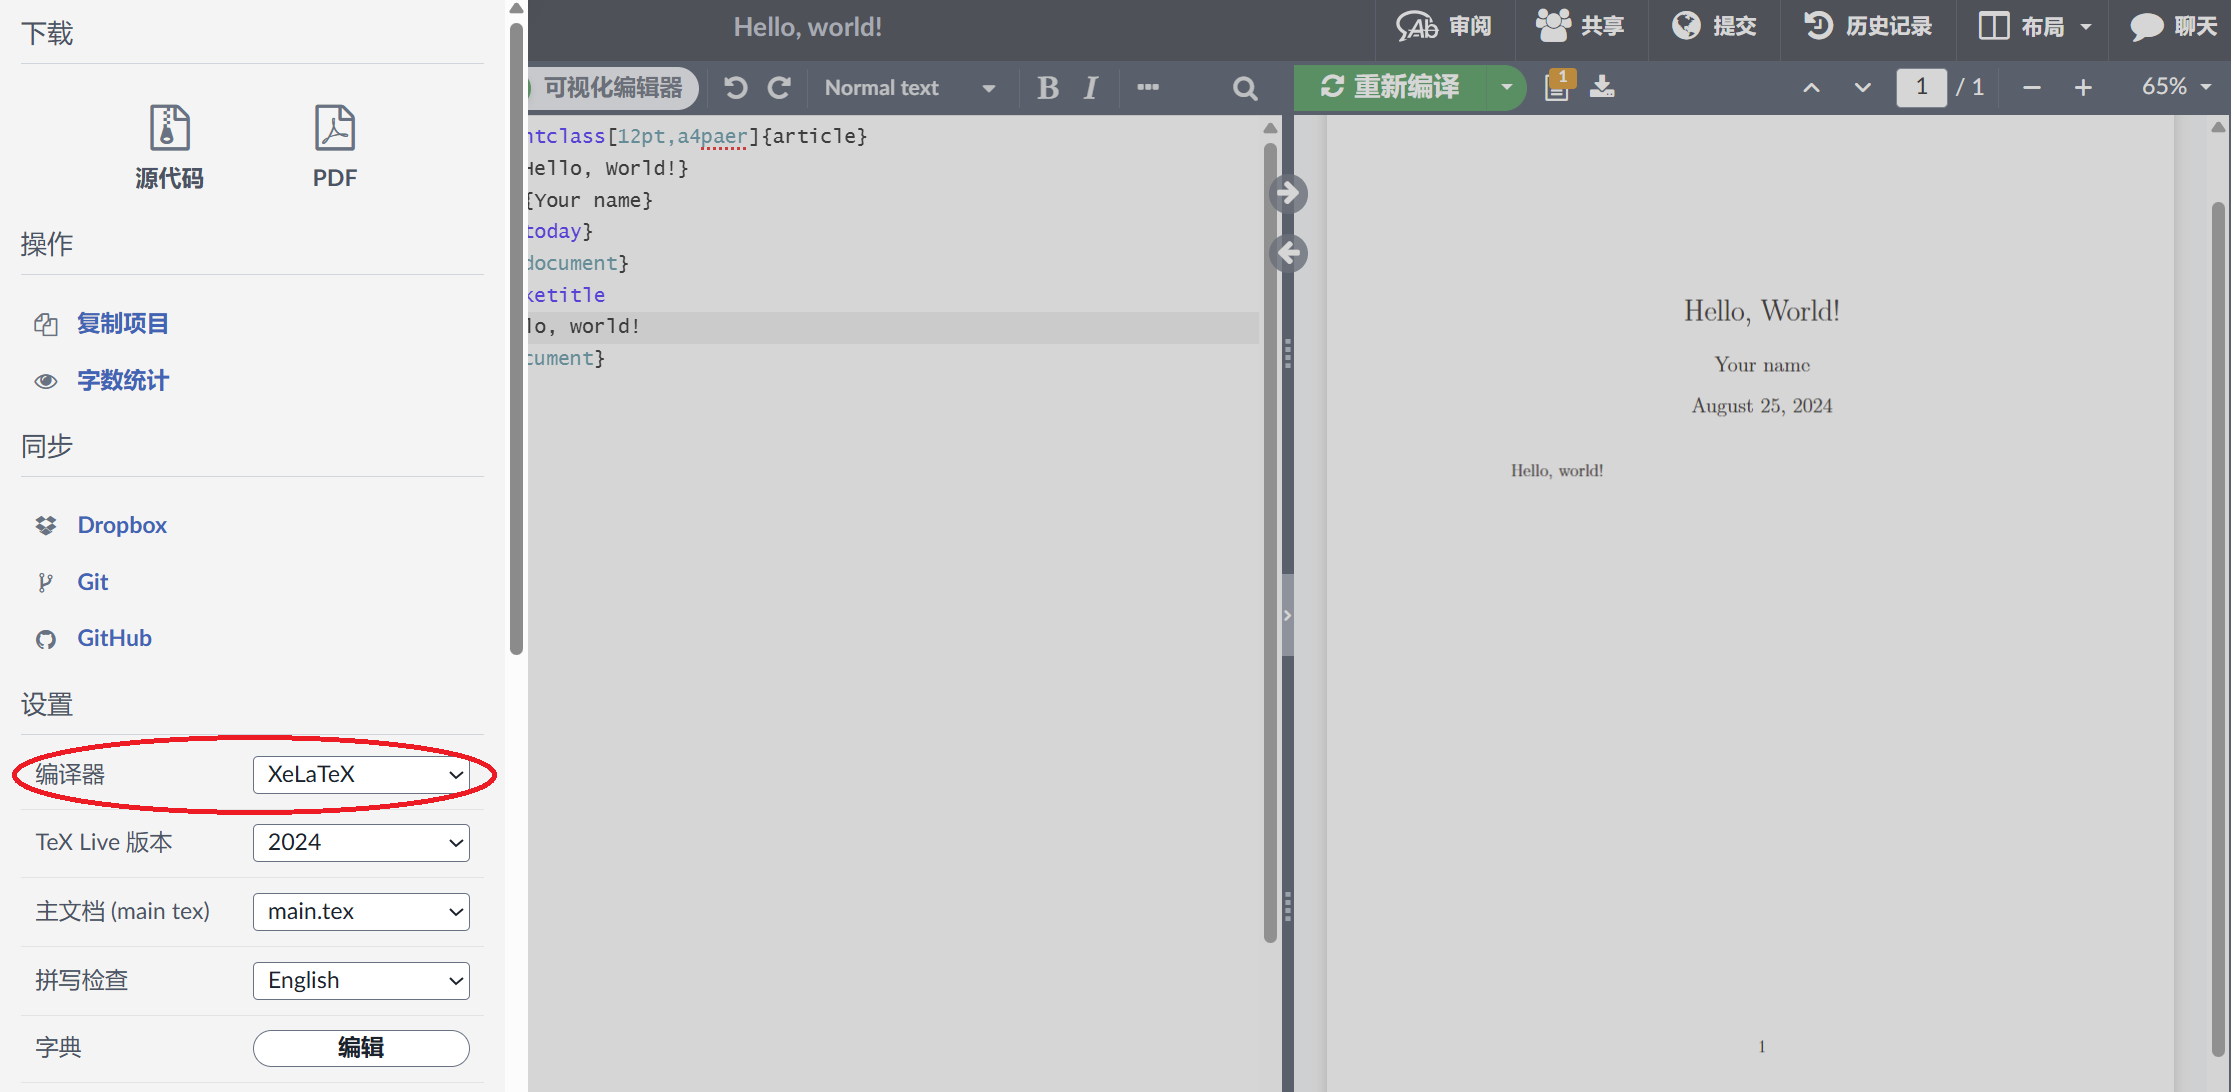
\includegraphics[width=0.8\textwidth]{figure/overleaf-compiler.png}
    \end{figure}
    然后可以点``重新编译''查看效果.
\end{frame}

\begin{frame}[fragile]
    \frametitle{控制序列}
    我们开始讨论\LaTeX{}的语法.
    一个典型的\textbf{控制序列} (control sequence) 形如
    \begin{lstlisting}
        \csname[option]{#1}
    \end{lstlisting}
    其中\Verb|\csname|是控制序列的名称, 花括号内的是控制序列作用的对象, 方括号内是参数.
    有时候后两者是不必要的.
    我们现在见过了控制序列\Verb|\documentclass[12pt]{article}|等, 接下来我们会仔细讨论它们的含义.
\end{frame}

\begin{frame}
    \frametitle{导言区}
    文档\Verb|Hello, World!|的导言区为
\end{frame}

\end{document}